\documentclass[11pt,a4paper]{article}
\usepackage[margin=2.2cm]{geometry}
\usepackage{amsmath,amssymb}
\usepackage{siunitx}
\usepackage{booktabs}
\usepackage{xcolor}
\usepackage{microtype}
\usepackage{enumitem}
\usepackage{tcolorbox}
\usepackage{graphicx}
\definecolor{ink}{HTML}{14231B}\definecolor{accent}{HTML}{0F3D2A}
\tcbuselibrary{skins}
\newtcolorbox{key}{colback=accent!6,colframe=accent,boxrule=0.6pt,arc=2pt,left=6pt,right=6pt,top=4pt,bottom=4pt}
\sisetup{per-mode=symbol,group-separator={\,}}
\setlength{\parindent}{0pt}\setlength{\parskip}{6pt}
\renewcommand{\arraystretch}{1.25}

\title{\textbf{Slide 3: input and bias-T}\\\large One coax carries the signal in and the power out}
\author{ADS7057 test board v3 \quad ---\quad study notes}\date{}
\begin{document}\maketitle\vspace{-1.2em}
\section{What the circuit must do}
The sensor head has no battery. It needs about \SI{4.3}{mA} of DC from the main board. The same coax must also bring the AE signal (100 to \SI{500}{kHz}) back, without the supply wires loading it. A \emph{bias-T} does this with two parts that behave in opposite ways:
\begin{itemize}[nosep]
\item an \textbf{inductor} passes DC and blocks AC ($|Z_L|=2\pi fL$),
\item a \textbf{capacitor} blocks DC and passes AC ($|Z_C|=1/2\pi fC$).
\end{itemize}
\begin{center}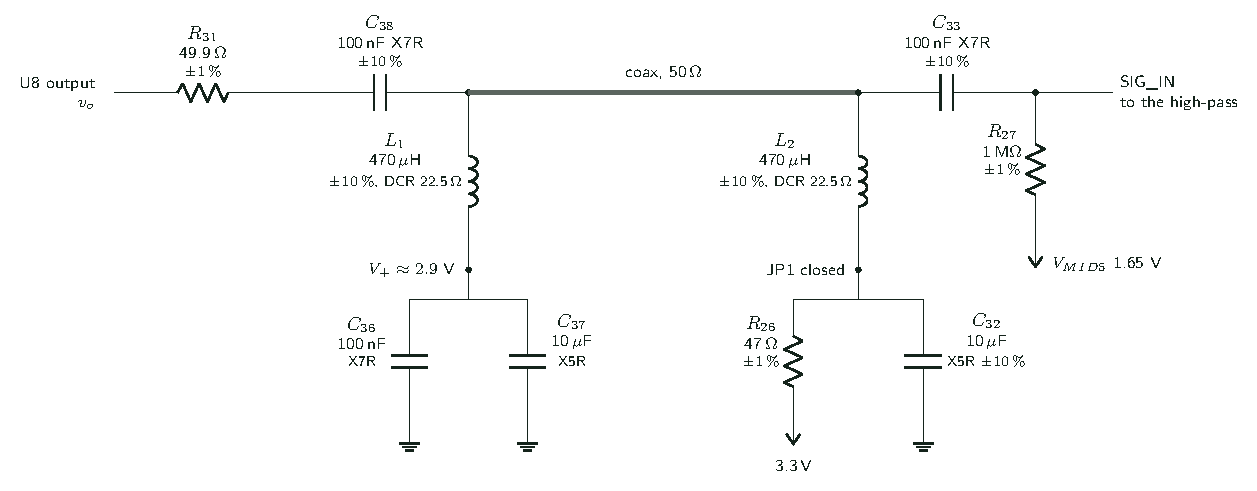
\includegraphics[width=0.98\textwidth]{s03_circuit.pdf}\end{center}

\section{The DC path: how much voltage reaches the head}
DC flows from $+3.3\,$V through R26, the closed jumper JP1, L2, the coax centre, and L1 into the head. At DC the capacitors are open and the inductors are only their winding resistance, DCR $=\SI{22.5}{\ohm}$ each (LCSC C75644). So
\[
R_\text{DC}=R_{26}+\mathrm{DCR}_{L2}+\mathrm{DCR}_{L1}=47+22.5+22.5=\SI{92}{\ohm},
\qquad
\Delta V=I\,R_\text{DC}=\SI{4.3}{mA}\times\SI{92}{\ohm}=\SI{0.40}{V},
\]
\[
V_+=3.3-0.40=\SI{2.90}{V}.
\]
This is the supply of the OPA365. The head amplifier works from 2.2 to \SI{5.5}{V}, so there is margin. The inductor is rated \SI{40}{mA}, ten times the load.

R26 and C32 form a supply filter with a corner at $1/(2\pi\cdot47\cdot10\,\mu\text{F})=\SI{339}{Hz}$. It removes ripple from the 3.3\,V rail before it enters the coax.

\section{The AC path: what the signal sees}
The head output drives R31 (\SI{49.9}{\ohm}) and C38. Both inductors hang from the coax line to an AC ground (their far ends sit on large capacitors). Two branches $Z_b=R_\text{DCR}+j\omega L$ are in parallel, so the line is loaded by
\[
Z_L=\tfrac12\,(R_\text{DCR}+j\omega L).
\]
The source impedance is $Z_s=R_{31}+1/(j\omega C_{38})$. The line voltage is a plain divider:
\[
H(s)=\frac{Z_L}{Z_L+Z_s}
=\frac{s^2\frac{LC}{2}+s\frac{R C}{2}}{s^2\frac{LC}{2}+s\,C\!\left(\frac R2+R_{31}\right)+1}.
\]
Read it as a \textbf{second-order high-pass} with
\[
\omega_0=\sqrt{\frac{2}{LC}},\quad f_0=\frac{1}{2\pi}\sqrt{\frac{2}{470\,\mu\text{H}\cdot100\,\text{nF}}}=\SI{32.8}{kHz},
\qquad
Q=\frac{1}{\omega_0\,C\,(R/2+R_{31})}\approx0.79 .
\]

\begin{key}
Below about \SI{33}{kHz} the inductors short the line to ground, so the bias-T rejects low-frequency noise by itself. At \SI{10}{kHz} the loss is \SI{18.5}{dB} by hand and \SI{18.7}{dB} in ngspice. At \SI{250}{kHz}, the middle of the AE band, the hand model gives about 0\,dB and ngspice gives \SI{0.17}{dB}. The extra 0.1\,dB comes from the cable and the filter loading, which the hand model leaves out.
\end{key}

\begin{center}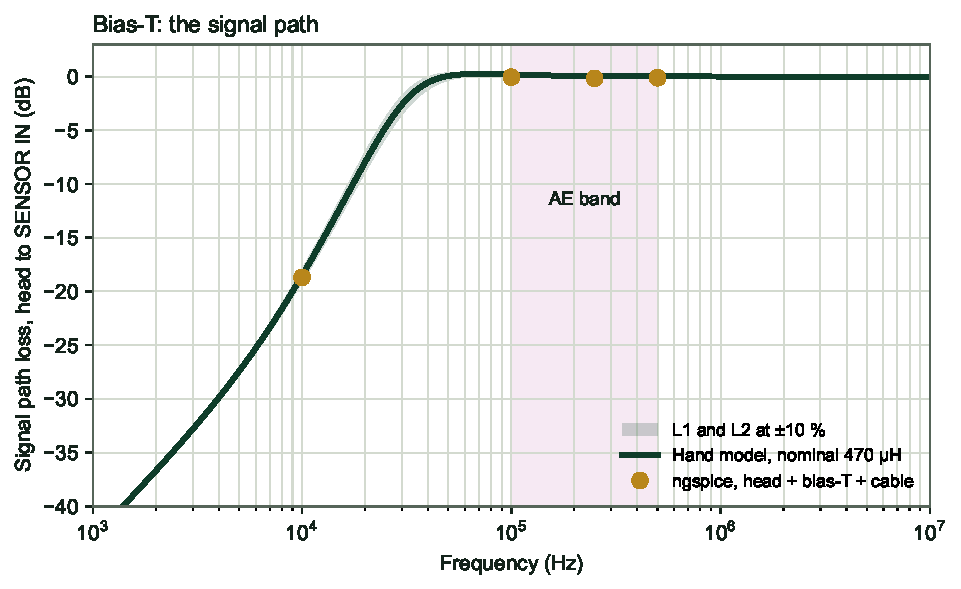
\includegraphics[width=0.78\textwidth]{s03_graph.pdf}\end{center}

\section{Checks and tolerances}
\begin{center}
\begin{tabular}{lll}
\toprule
Item & Value & Effect\\
\midrule
L1, L2: 470\,\textmu H $\pm10\,\%$ & $f_0$ moves $\pm5\,\%$ (31 to \SI{34.5}{kHz}) & small, shown as the grey band\\
Wavelength at \SI{250}{kHz} & about \SI{800}{m} in the cable & a 1\,m cable is a lumped element\\
Cable capacitance (RG174, about \SI{100}{pF/m}) & \SI{6.4}{k\ohm} at \SI{250}{kHz} & adds a small load\\
Inductor self-resonance & \SI{2}{MHz} & above the band, so $L$ stays an inductor to \SI{500}{kHz}\\
C33 and R27 at SIG\_IN & \SI{100}{nF} into \SI{1}{M\ohm} & $\SI{1.6}{Hz}$ corner, DC blocked\\
\bottomrule
\end{tabular}
\end{center}
\end{document}
